\section{Bots and AI}

\begin{figure}
    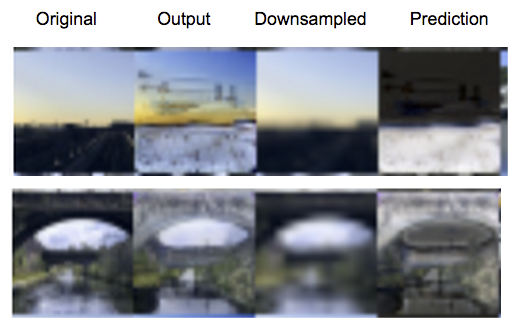
\includegraphics[width=\linewidth]{05_GANs/eyescream_predicted16.png}
    \caption{Skyline and bridges, generated by Eyescream (2015)}
    \label{fig:eyescream}
\end{figure}

\begin{figure}
    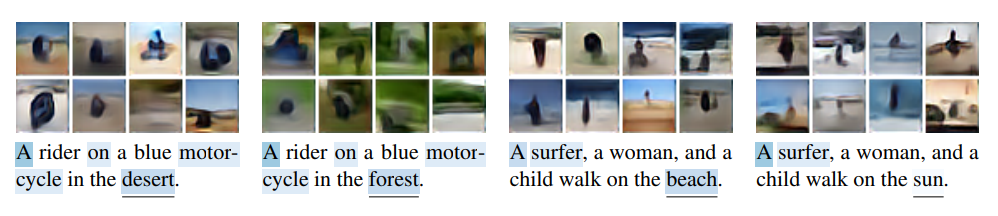
\includegraphics[width=\linewidth]{05_GANs/gen_from_captions.png}
    \caption{Example of most attended words while changing the background}
    \label{fig:gen_attention}
\end{figure}

\begin{figure}
    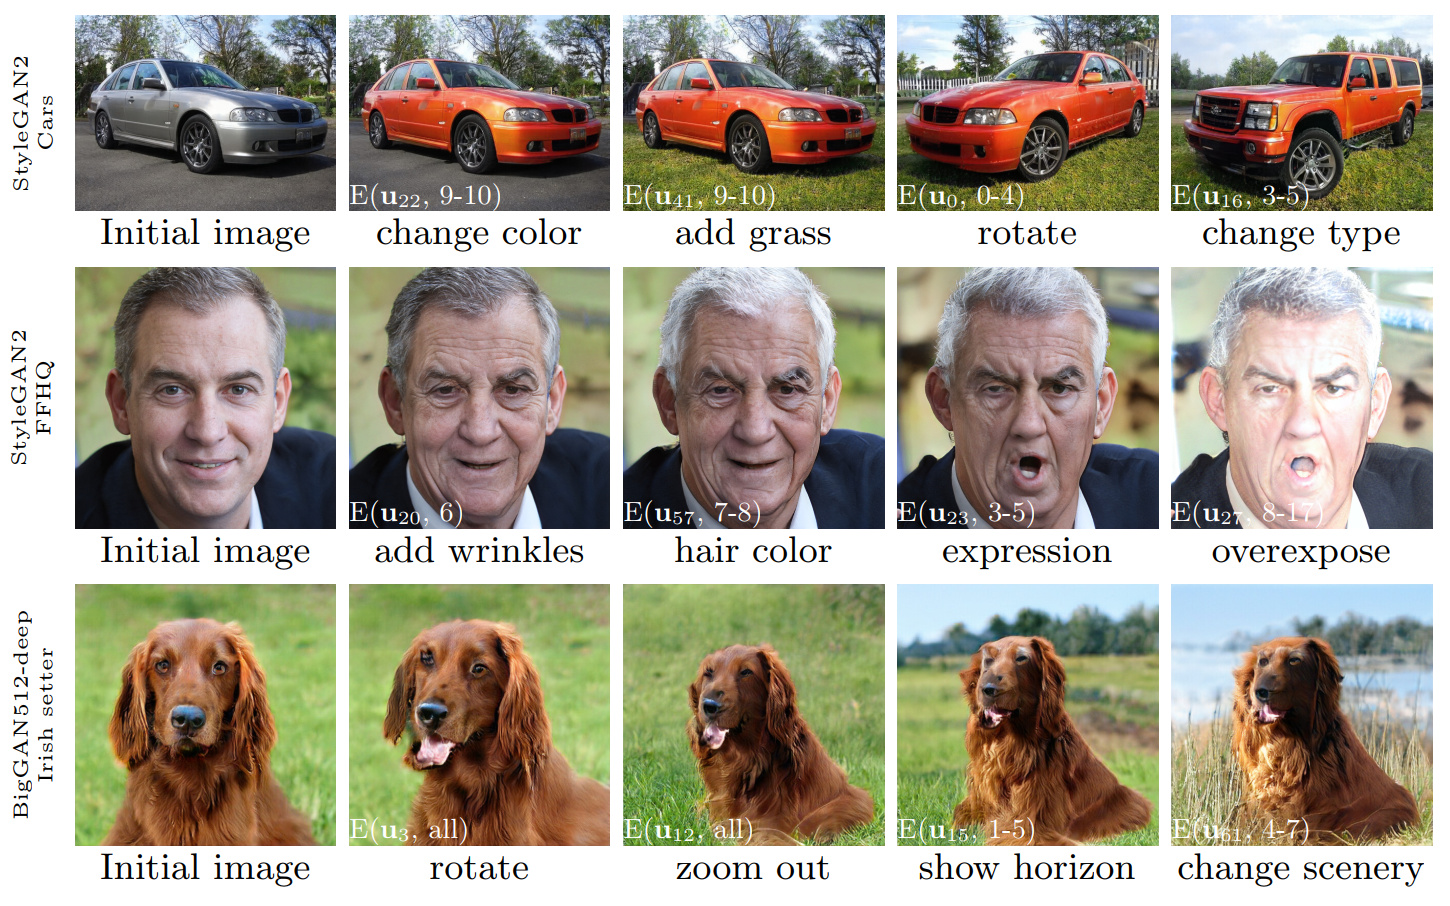
\includegraphics[width=\linewidth]{05_GANs/ganspace.jpg}
    \caption{Sequences of image edits performed using control discovered with GANSpace, applied to three different GANs.}
    \label{fig:ganspace}
\end{figure}

\begin{figure}
    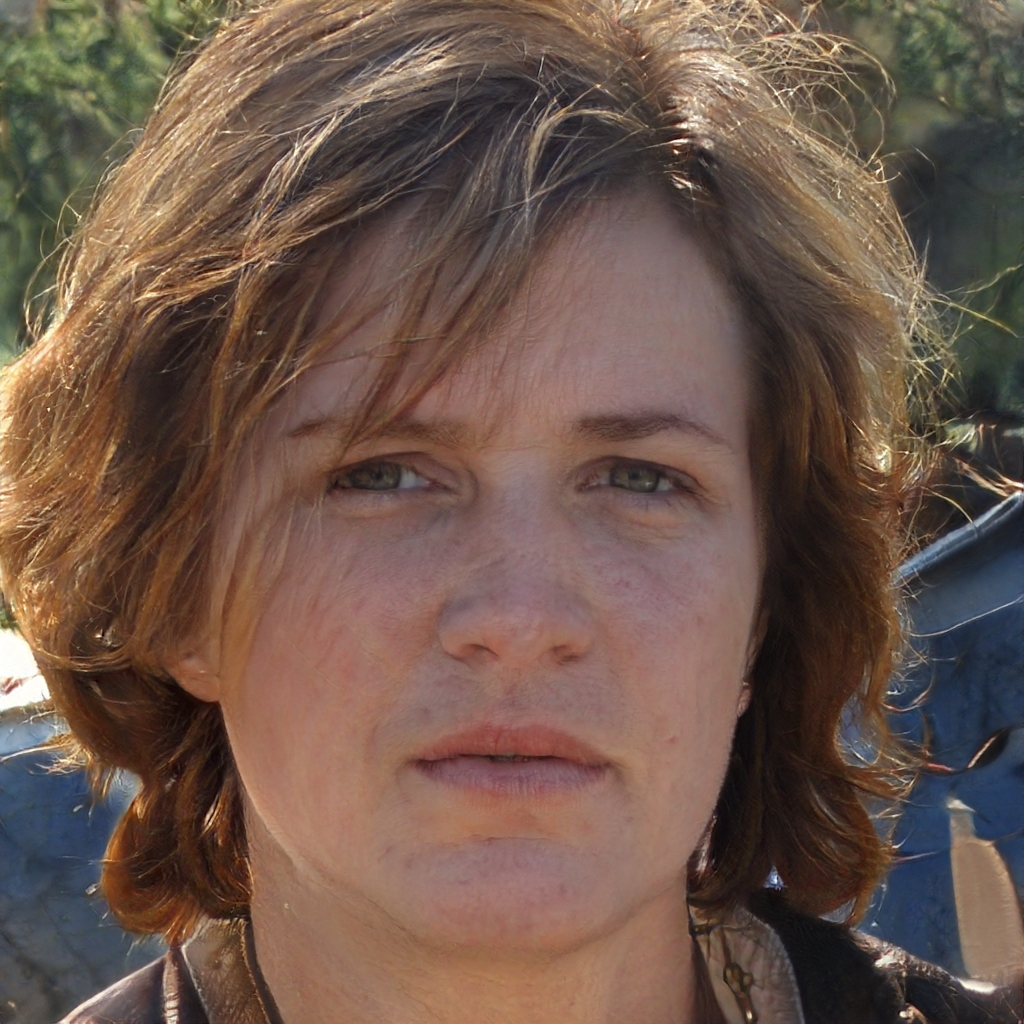
\includegraphics[width=0.5 \linewidth]{05_GANs/joiseocampbell.jpg}
    \caption{Josie O. Campbell: a fake person generated by an AI}
    \label{fig:fakeperson}
\end{figure}

Around 2014, Generative Adversarial Networks, a type of neural network designed by Ian Goodfellow and his team \cite{goodfellow2014generative}, was introduced. The next year, Batch Normalization \cite{ioffe2015batch} and the definition of Residual Networks \cite{he2015deep} was born. These, amongst many more discoveries up until today allowed neural networks to deeper, more efficiently, and with much better results.

One paper from 2015 \cite{denton2015deep} shows outstanding --for the time-- results in terms of image generation using GANs. From a very low quality image, the network is able to generate a completely new image, either reconstructing the original, or coming up with its own interpretation of the available data (Figure \ref{fig:eyescream}). The same year, another team in Toronto developed a neural network that could generate images from a natural language text description (Figure \ref{fig:gen_attention}). This was merely the start of the GAN revolution.

More recent studies allow GANs to be use parameters that can be tuned to generate specific variants of the same output image. An example is the image of the face of a person, that smiles or frowns, according to a given parameter, or turns its head left and right, or has glasses on or off, see Figure \ref{fig:ganspace}.

These advancements looked great, as they served to push the advancements in the field much forward. As the development in this field progressed, more discoveries were made, and higher quality images could be reproduced. 

However, with more advanced and real-looking outputs, comes different problems. In Chapter \ref{chap:rise_fake} for example, we started by describing a woman in her forties using a generated output from a website. Of course, if you were browsing a Facebook page or an online forum with her profile, you would think twice about her being real. No pictures of her, and her connections are also without a profile picture. Suspicious.

With GANs however, we can give good ol' Josie Campbell a face, like the one in \ref{fig:fakeperson} generated using the output of a website called \href{https://thispersondoesnotexist.com}{ThisPersonDoesNotExist.com}. The site uses a GAN architecture called \textit{StyleGAN2} \cite{karras2020analyzing}, which greatly outperforms the previous architecture \textit{StyleGAN} \cite{karras2019stylebased} in terms of quality and realness.

Now that Josie Campbell has a face of her own, even though it is fake, she suddenly became much more credible, and you wouldn't question right away that she isn't a real person.

Suddenly, we have created a person from thin air, and she can write and do whatever we please. She can be a woman that fights for human rights, or she can be an advocate for Donald Trump's latest fake news about the Democrats.

In Section \ref{chap:clickfarms} we talked about click farms, and the people who work in them. They are being paid incredibly little to operate up to two hundred phones each. Now, imagine the impact of pictures generated by GANs can have in the creation of new accounts. For every account you can have a totally different person, with a unique set of traits and pictures.

It would be incredibly hard for social media algorithms to filter and block such activities, as they look so real at a first glance, even for manual reviews.

If you throw fake news into the mix, you can possibly lead an army of online accounts that fight for your points of views and beliefs. You can possibly fool the popular opinion by generating thousands of people that will talk about your cause, whatever that might be. 

What if you want to take a step forward, and generate a video that shows them doing some common activities, like walking or skiing? This can be done, with some limitations, with the use of ``DeepFakes'' \cite{Suwajanakorn2017SynthesizingO, thies2020face2face}. This is a recent technique where the face of a person in a video is replaced by another one, imitating their expressions and poses. Features that put this method under the spotlights, both for their incredible results, and their potential consequences.

Suddenly, you could make Obama the starring character of the movie ``300'', or make fun of a friend by pasting his face into some viral video. Or you could change the face of a porn video actress to someone else's face.

It started to become obvious that Deepfakes were not a tool for funny jokes and memes anymore, but they could become a way to bully and blackmail. In fact, this technique also applies to all kinds of objects, not only faces. In 2019, a group of researchers in Israel proved that you could also change the outcome of a CT scan \cite{Hospital63:online}, perhaps injecting a fake cancerous nodule into someone's lung's output image.

As the cherry on top, OpenAI, one of world's leading AI-focused companies, released in June 2020 a software called GPT-3 \cite{brown2020language}. This AI model is able to do incredible things, from powering a text-based game called AI-Dungeon \cite{AIDungeo6:online}, to writing essays able to score a C \cite{WhatGrad58:online}. The GPT-3 model is not easily available to the public, and for good reasons. Just imagine the level of detail and stories that this technology could create, from blog articles to populating a profile's \textit{Facebook Wall} of realistic interactions.
